\begin{ledgroupsized}[r]{120mm}
\footnotesize 
\pstart                
\noindent\textbf{\"{U}berlieferung:}   
\pend
\end{ledgroupsized}
\begin{ledgroupsized}[r]{114mm}
\footnotesize 
\pstart \parindent -6mm
\makebox[6mm][l]{\textit{L}}%
Auszüge mit Bemerkungen aus einem verschollenen Manuskript
von René Descartes:\protect\index{Namensregister}{\textso{Descartes} (Cartesius, des Cartes), Ren\'{e} 1596-1650}
LH~IV 1, 4b Bl. 3-12.
5~Bog. 2\textsuperscript{o}.
Etwa 18 S.
Bl. 6~v\textsuperscript{o} nur zu \nicefrac{2}{3} beschrieben,
Bl. 12~r\textsuperscript{o} nur zur Hälfte,
Bl.~12~v\textsuperscript{o} leer.
Sämtliche Bog. von Leibniz durchnummeriert.
Kustoden am unteren Rand von Bl. 4~v\textsuperscript{o}, 6~v\textsuperscript{o}, 8~v\textsuperscript{o} und 10~v\textsuperscript{o}.
% Text durch Überschriften in 6 Abschnitte gegliedert.
Im unteren Sechstel von Bl. 10~r\textsuperscript{o} und von Bl. 10~v\textsuperscript{o} ist N.~6 % LH 004,01,04b_009-010 = Aus und zu Athanasius Kircher, Magnes
überliefert.
Für einzelne Passagen aus dem verschollenen Manuskript
%\textit{In eo convenit formatio plantarum} [...] \textit{lien vero 2 diebus intermissis} 
besteht eine parallele Überlieferung in \cite{01144}\textsc{R.~Descartes}, \textit{Opuscula posthuma}, Amsterdam 1701, \glqq Primae co\-gi\-ta\-tio\-nes circa generationem animalium\grqq~%
(siehe unten, S.~\refpassage{004_01_04b_009r_pU1a}{004_01_04b_009r_pU1b}; S.~\refpassage{004_01_04b_009r_pU2a}{004_01_04b_009r_pU2b};  S.~\refpassage{004_01_04b_009r_pU3a}{004_01_04b_009r_pU3b}; S.~\refpassage{004_01_04b_009r_pU4a}{004_01_04b_009r_pU4b}).
\newline%
% Wegen ihres komplexen Characters erfolgt die Wiedergabe der Figuren als Schema-Zeichnung und als Reproduktion des Originals, um lesbare Transkription und notwendige N\"{a}he zum Original zu erreichen.
Cc 2, Nr. 1322 A-E (D tlw.)
\pend
\end{ledgroupsized}
% \vspace*{0.5em}
%
\begin{ledgroupsized}[r]{114mm}
\footnotesize 
\pstart \parindent -6mm
\makebox[6mm][l]{\textit{E\textsuperscript{1}}}%
% (tlw.) 
\cite{01121}\textsc{R. Descartes}, \textit{{\OE}uvres in\'{e}dites}, hrsg. von \textsc{L.A. Foucher de Careil}, 2 Bde, Paris 1859- 1860, Bd. I, S. 100-155; Bd. II, S. 66-209 (in verschiedener Reihenfolge; mit franz\"{o}sischer \"{U}bersetzung).
\pend
\end{ledgroupsized}
% \vspace*{0.5em}
%
\begin{ledgroupsized}[r]{114mm}
\footnotesize 
\pstart \parindent -6mm
\makebox[6mm][l]{\textit{E\textsuperscript{2}}}%
\cite{00120}\textsc{R. Descartes}, \textit{{\OE}uvres}, hrsg. von \textsc{C. Adam} und \textsc{P. Tannery}, Bd. XI, Paris 1909, S.~534-538, 549-621.
\pend
\end{ledgroupsized}
%
%\normalsize
\vspace*{5mm}
\begin{ledgroup}
\footnotesize 
\pstart
\noindent\footnotesize{\textbf{Datierungsgr\"{u}nde:}
Siehe die für das Stück N.~54
% LH004,01,04b_013-014 = Ex Manuscripto Cartesii. Problemata
angeführten Datierungsgründe.
}%
\pend%
\end{ledgroup}%
%
\vspace*{8mm}%
\count\Bfootins=1200
\count\Cfootins=1200
\count\Afootins=1200
\pstart
\noindent [3~r\textsuperscript{o}]
\pend
\pstart%
\normalsize%
\noindent%
\centering% PR: Bitte als Überschrift gestalten.
% [3~r\textsuperscript{o}]
Anatomica quaedam ex Mso Cartesii\protect\index{Namensregister}{\textso{Descartes} (Cartesius, des Cartes), Ren\'{e} 1596-1650}%
\edtext{}{\lemma{}\Afootnote{\textit{Am Rand:} (I.)\vspace{-6mm}}}
\pend%
\vspace*{1.0em}% PR: Rein provisorisch !!!
\pstart%
\noindent%
In corde vitulino a me dissecto haec observavi. 1\textsuperscript{o} paries medius inter utrumque ventriculum positus erat omnium Densissimus, \edtext{pariesque dextri}{\lemma{pariesque}\Bfootnote{\textit{(1)}\ sinistri \textit{(2)}\ dextri \textit{L}}} lateris erat densior quam sinistri, adeo ut hi tres se proportione quadam sequerentur. 
\pend 
\newpage
\pstart  Ex inferiore parte uniuscujusque sinus erat unum vas, cujus tunicae \edtext{substantia non}{\lemma{substantia}\Bfootnote{\textit{(1)}\ nonnihil \textit{(2)}\ non \textit{L}}} multum ab ipsius cordis substantia differre videbatur, nec multum ab invicem, tunicae aderant satis tenues, haec vasa credidi esse in sinistro arteriam venosam, in dextro venam cavam, neque unum altero majus videbatur, nec satis distincte illorum valvulas agnoscebam, tamen erant
\edtext{[illarum]}{\lemma{illorum}\Bfootnote{\textit{L \"{a}ndert Hrsg.}}}
vestigia, membrana enim sinus cordis obducens in vasium ingressu desinebat in fibras, versus cuspidem parietibus adhaerentes, haeque fibrae tenacius adhaerebant, in sinistri sinus duobus locis, et dextri tribus, ut quod per illa vasa ingrederetur in cor, tam facile regredi non posset.
Notavi praeterea haec duo vasa in cordis \edtext{ingressu sibi}{\lemma{ingressu}\Bfootnote{\textit{(1)}\ sui \textit{(2)}\ sibi \textit{L}}} invicem esse communia nec separari nisi membrana tenuissima et laxissima, quae utrinque flecti poterat, erat autem in infima parte adhuc aperta (vel forte a me imprudenter rupta) et videbatur ex illa parte quae aperta erat e vena cava in arteriam venosam humor delabi posse, non contra. Si autem superior pars istius membranae rupta fuisset, tunc potuisset humor ex arteria in venam effluere, non contra; utrinque autem super ista duo vasa erant productiones laxae et cavernosae sursum flexae, quas auriculas vocant, non dissimilis substantiae ac ipsa vasa, ut ibi essent tantum quasi sinus, in quibus humor, qui in cor ingredi non poterat, congerebatur (notant etiam anatomici illas contrarium habere motum motui cordis), nec inter utramque aliam differentiam  \edtext{notavi, nisi}{\lemma{notavi,}\Bfootnote{\textit{(1)}\ quam \textit{(2)}\ nisi \textit{L}}} quod essent plures anfractus in sinistrae cavitatibus quam in dextrae, sinistraeque membrana alba interior magis alba erat et densa quam dextrae. Illarum anfractus eos qui sunt in sinubus cordis referebant (: adeo, ut 
 \begin{wrapfigure}[13]{l}{0.3\textwidth}
\vspace{-2mm}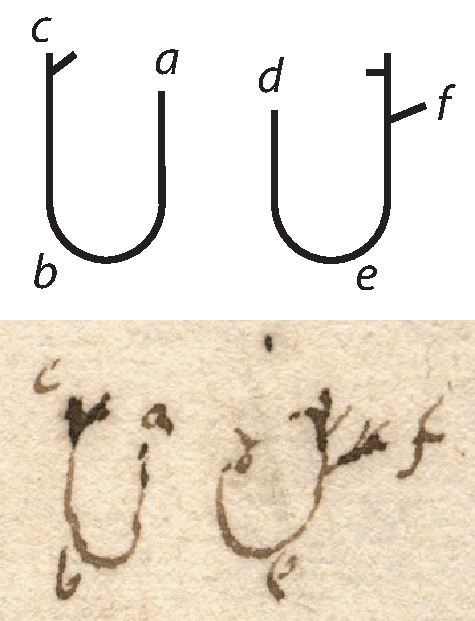
\includegraphics[trim = 0mm -3mm -5mm 0mm, clip, width=0.3\textwidth]{images/lh0040104b_003r1.pdf}\\
\rule[0cm]{14mm}{0cm}[\textit{Fig. 1}]
%\caption{Bildbeschreibung}
\end{wrapfigure}
videatur initio produci duos sinus ab arteria venosa, et duos a cava, ex quibus duo sive sinistri sive inferiores simul uniuntur faciunt cor, alii duo ab invicem separati, auriculas. :) Jam sinus sinister longior erat dextro et angustior desinebatque in aortam. $a$  arteria venosa, $b$ cuspis cordis, $c$ aorta et dexter in venam arteriosam. $d$ cava. $e$ cuspis cordis. $f$ vena arteriosa. Paries sinistri ad sinum usque cordis pertingebat, ubi non erat admodum crassus paries dextri prius desinebat sed majorem basis partem amplectebatur, (nempe
\edtext{[$df$]}{\lemma{$bf$ }\Bfootnote{\textit{L \"{a}ndert Hrsg.}}}
est major quam $ac$) ideoque $c$ tanquam ex medio basis surgebat et $f$ illam amplectebatur. Membrana sinus sinistri erat, magisque alba et densa quam dextri; fulciebantur vero isti sinus aliquibus quasi columnis e medio pariete versus basin in externos parietes versus cuspidem tendentibus quae licet paucae essent et promiscue sitae, erant tamen valde rotundae; et ex similibus totus \edtext{cor}{\lemma{}\Afootnote{\textit{\"{U}ber} totus cor: \Denarius}} conflatus videbatur, \edtext{ut}{\lemma{}\Afootnote{\textit{Am Rand:} \Denarius}} apparebat ex multis rimis utrinque in parietibus. 
\pend 
\count\Bfootins=1500
\count\Cfootins=1500
\count\Afootins=1500
\pstart  Jam sursum aorta et vena arteriosa se mutuo tangebant ut infra aliae duae, sed nullam habebant inter se communicationem valvulas distincte in illis vidi quales describuntur et intervallum inter 2\textsuperscript{as} valvulas aortae, e regione respondebat intervallo inter duas valvulas venae arteriosae, et immediate supra duas valvulas aortae, quae viciniores erant venae arteriosae, vel potius intra ipsas valvulas duo erant exigua foramina, quae ostendebant quasi duos ramos aortae, quibus utrinque venam arteriosam amplectebatur, iique rami rursus in cor absumebantur non autem apparebat ulla communis via inter aortam et venam arteriosam, sed una ab altera poterat tota divelli, neutra etiam videbatur, altera multo major, vel substantiae diversae, sed utraque erat densissima, alba \edtext{autem}{\lemma{autem}\Bfootnote{\textit{erg. L}}} et quasi cordi implantata, non ejus substantiam constituens, ut vasa inferiora. \pend 
\pstart  Erat etiam adeps exteriori superficiei cordis versus basin multis in locis adnata, ut et tunicae aortae, et venae arteriosae videbantur magis exteriori parti cordis quam interiori adnatae, quod contrarium erat in vena cava, et arteria venosa, quae omnia rationibus meis \edtext{tam}{\lemma{}\Afootnote{\hspace{-1.8mm}\textit{Am Rand:} (+ NB +)\vspace{-4mm}}} accurate conveniunt ut nihil magis.
\pend 
\pstart  Valvularum interstitia ad venam cavam unum erat in medio parietis externi ventris dextri per fibras ex crassiusculo quodam tuberculo exeuntes, alia duo erant in lateribus medii parietis. Fibrae dispergentes valvulas arteriae venosae erant in utroque latere parietis externi ventris sinistri, nullae in medio pariete. 
\pend 
\pstart  Valvulae autem aortae et venae arteriosae non erant in ipso corde, sed membranulae ex corde ad vasa emergebant, haerebantque utrinque uno interstitio super parietis medii dimidium, sibi invicem e regione correspondentes aliae 4 utrinque duae erant in lateribus simul aequali ab invicem distantia. Foris apparebat notabilis sutura, ventrem unum ab alio distinguens, instar venae cujus\-dam, quae etiam per medium parietem penetrare videbatur, ita ut ejus crassitiem quodammodo divideret. 
\pend 
\newpage
\pstart  Sed praeterea notavi ex arteria venosa, non unam tantum, sed quasi duas auriculas emergere unam secui quae vulgo notatur ab omnibus, aliam vero, quae in laxa illa valvula quae arteriam venosam a cava dividit absorbetur, et a trunco cavae ascendente contegitur. 
\pend
%\newpage
\pstart\noindent Duae autem verae auriculae habent extremitates suas, non una in aliam alia in alteram partem, sed utraque in sinistrum latus deflexas.
[3~v\textsuperscript{o}]
\pend